\section*{Background}

Substituted aromatic amines are essential intermediates involved in the synthesis of many pharmaceutical compounds, agrochemicals, and dyes \cite{vogt_amines_2000}. However, producing them directly through electrophilic aromatic substitution of the amino group is not possible, hence it is introduced via nitration and subsequent reduction \cite{dugal_nitrobenzene_2005}. Nitration poses major safety risks, and recent deadly industrial accidents on batch nitration plants such as the 2019 Xiangshui plant explosion, have prompted Chinese authorities to strengthen plant control and management \cite{el_diario_china_2019}. Furthermore, global chemical firms, for whom most plants in China produce intermediates, are being urged to source their raw materials more responsibly \cite{stanway_global_2019}.
In this context Nitroma, a foreign-invested enterprise, seeks to develop an inherently safer nitration process to produce substituted aromatics amines in China's growing market. Nitroma plans offer a socially responsible alternative to current suppliers for multinational firms eager to improve their environmental credentials. 

Recent developments in flow chemistry and process intensification enable the inherently safer design of industrial-scale nitration. Nitroma will profit from the transition to continuous nitration to safely manufacture important intermediates on a large-scale of over \SI{100}{\tonne\per\year} \cite{di_miceli_raimondi_safety_2015}. Using multi-criteria decision methods, the optimal combination of amino derivatives of toluene to be produced by Nitroma has been determined: 4-aminobenzaldehyde, a precursor of pharmaceuticals and vanillin, \ortho-toluidine, an intermediate in the manufacture of herbicides, and 4-aminobenzoic acid, an essential building block for the production of vitamin B9 \cite{bowers_toluidines_2000,bruhne_benzaldehyde_2011,maki_benzoic_2000}.
Nitroma's production capacity is flexible and adjustable to market demand. Modularity is built-in to the process, which can control the partial oxidation of \para-nitrotoluene to its benzaldehyde or benzoic acid derivatives. Based on current customer demand, the plant will initially operate a 240-day 4-aminobenzaldehyde campaign and a 35-day 4-aminobenzoic acid campain; capable of yielding \SI{652}{\tonne\per\year} of \SI{99}{\percent} pure \ortho-toluidine, \SI{538}{\tonne\per\year} of \SI{99.3}{\percent} pure 4-aminobenzaldehyde and \SI{100}{\tonne\per\year} of pure 4-aminobenzoic acid.

\begin{wrapfigure}{r}{0pt}
    \centering
    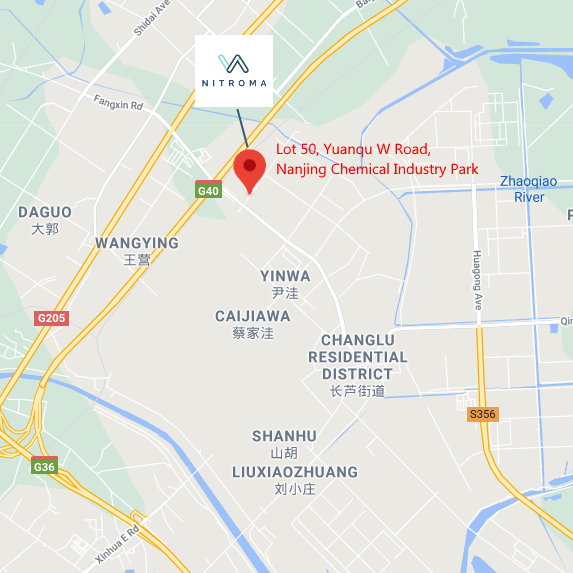
\includegraphics[width=0.2\linewidth]{chapters/0-executive-summary/figures/Location-crop.png}
    \caption{Nitroma's location}
    \label{fig:location}
\end{wrapfigure}
Nitroma's demonstration plant is located in the Nanjing Jiangbei New Material Science Park in Jiangsu (China). In addition to secured feedstock supply from China’s largest toluene manufacturer, Sinopec Yangzi Petrochemical, the Industry Park hosts all the necessary utilities and is well connected to main transportation hubs, thus guaranteeing that products can easily be shipped internationally []. 
This report details the initial design of Nitroma's plant, obtained following Process Intensification and Green Chemistry principles to develop an inherently safer and environmentally friendly continuous process.



